\xsection{myblue}{Introduction}

\begin{frame}
  \frametitle{Higgs-BRs all-in-one}
  \setbeamercovered{transparent}
  Trying to adapt a $\tau$ branching ratio \href{https://arxiv.org/abs/hep-ex/0506072}{\color{llblue} paper} from ALEPH to Higgs at ILD:
  \begin{columns}[c,onlytextwidth]
  \begin{column}{0.55\textwidth}
  \vfill
  \begin{enumerate}
    \item Build a (Higgsstrahlung) sample with all Higgs decay modes present.
    \item<2-> Construct categories to separate the decay modes (\& background) as well as possible.
    \item<4-> Fit the Higgs branching ratios to the observed category counts.
  \end{enumerate}
  \end{column}
  \begin{column}{0.45\textwidth}
  \only<1>{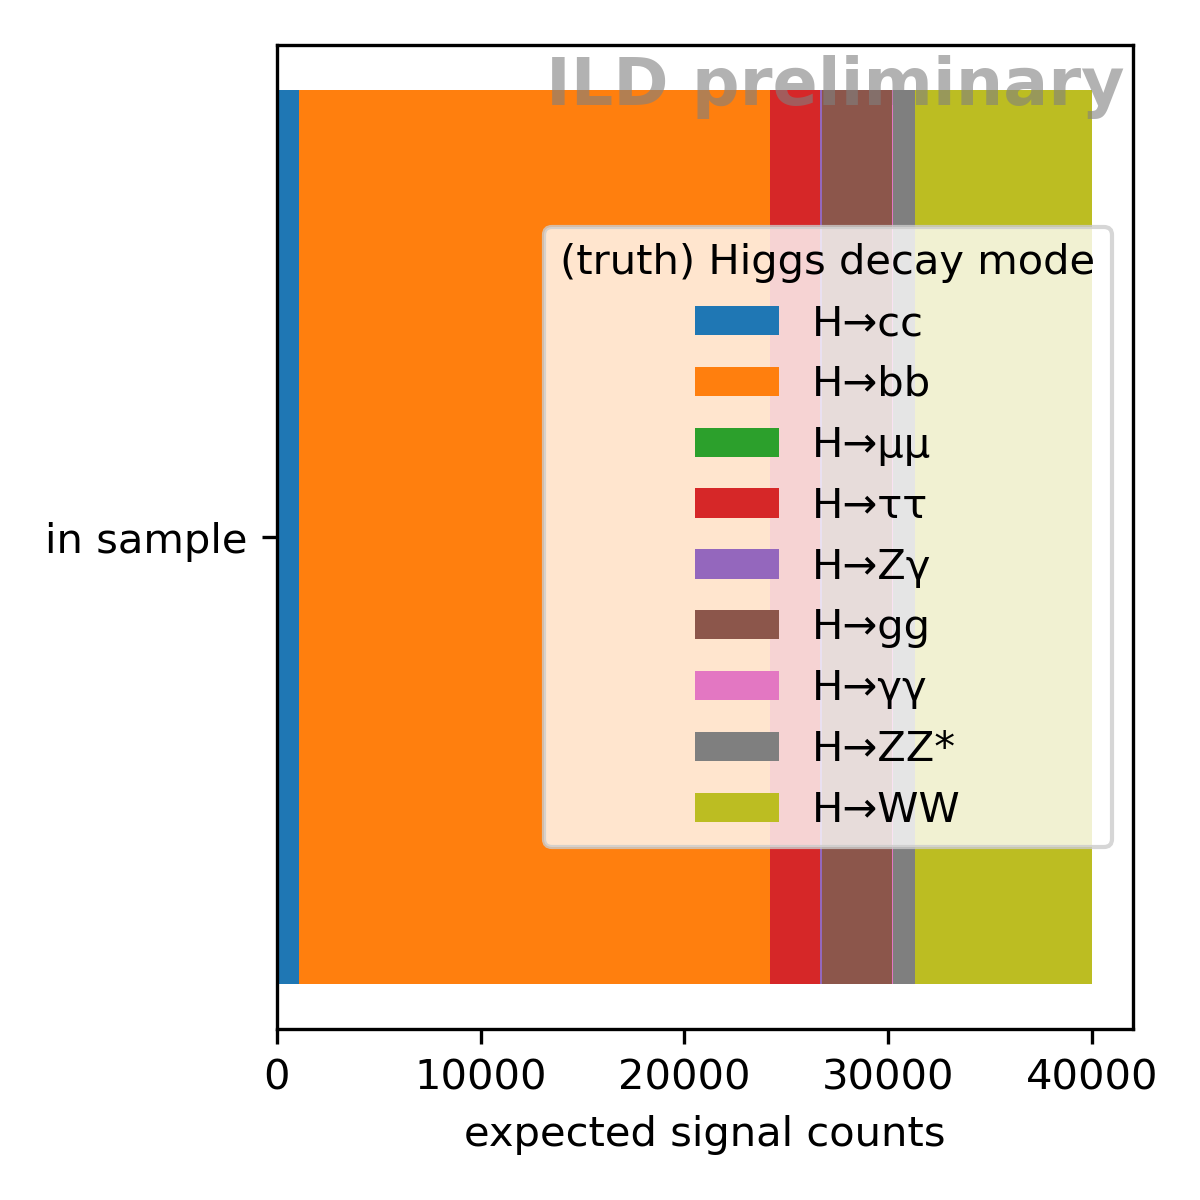
\includegraphics[height=0.85\textheight, width=0.95\textwidth, keepaspectratio]
      {plot_factory/intro_sample_counts}}
  \only<2>{\addtocounter{framenumber}{1} 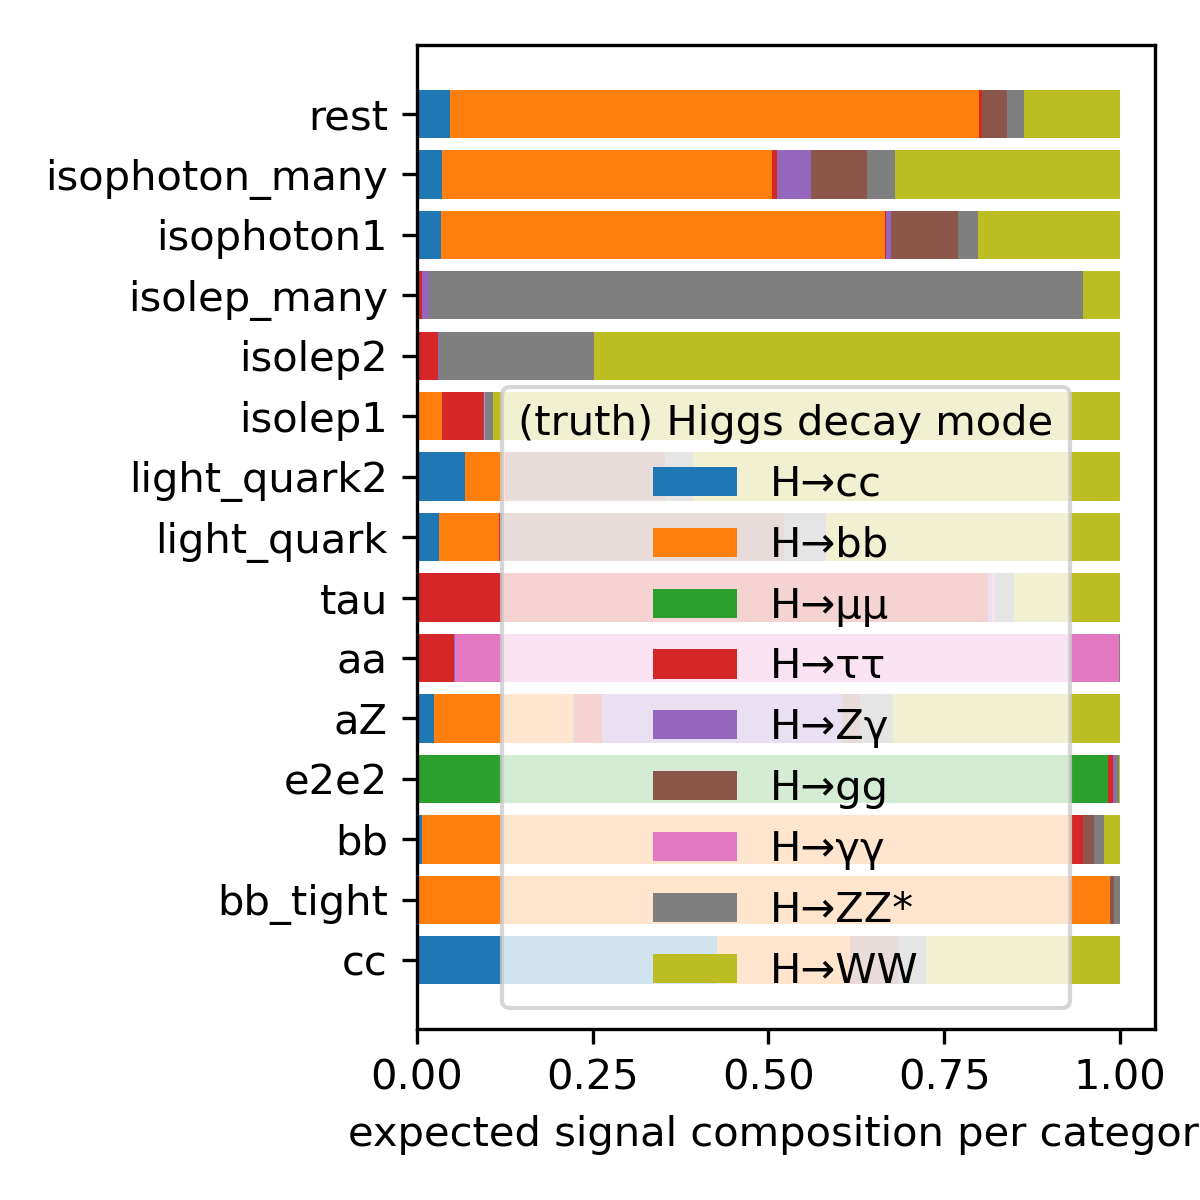
\includegraphics[height=0.85\textheight, width=0.95\textwidth, keepaspectratio]
      {plot_factory/intro_signal_composition_per_category}}
  \only<3>{\addtocounter{framenumber}{1} 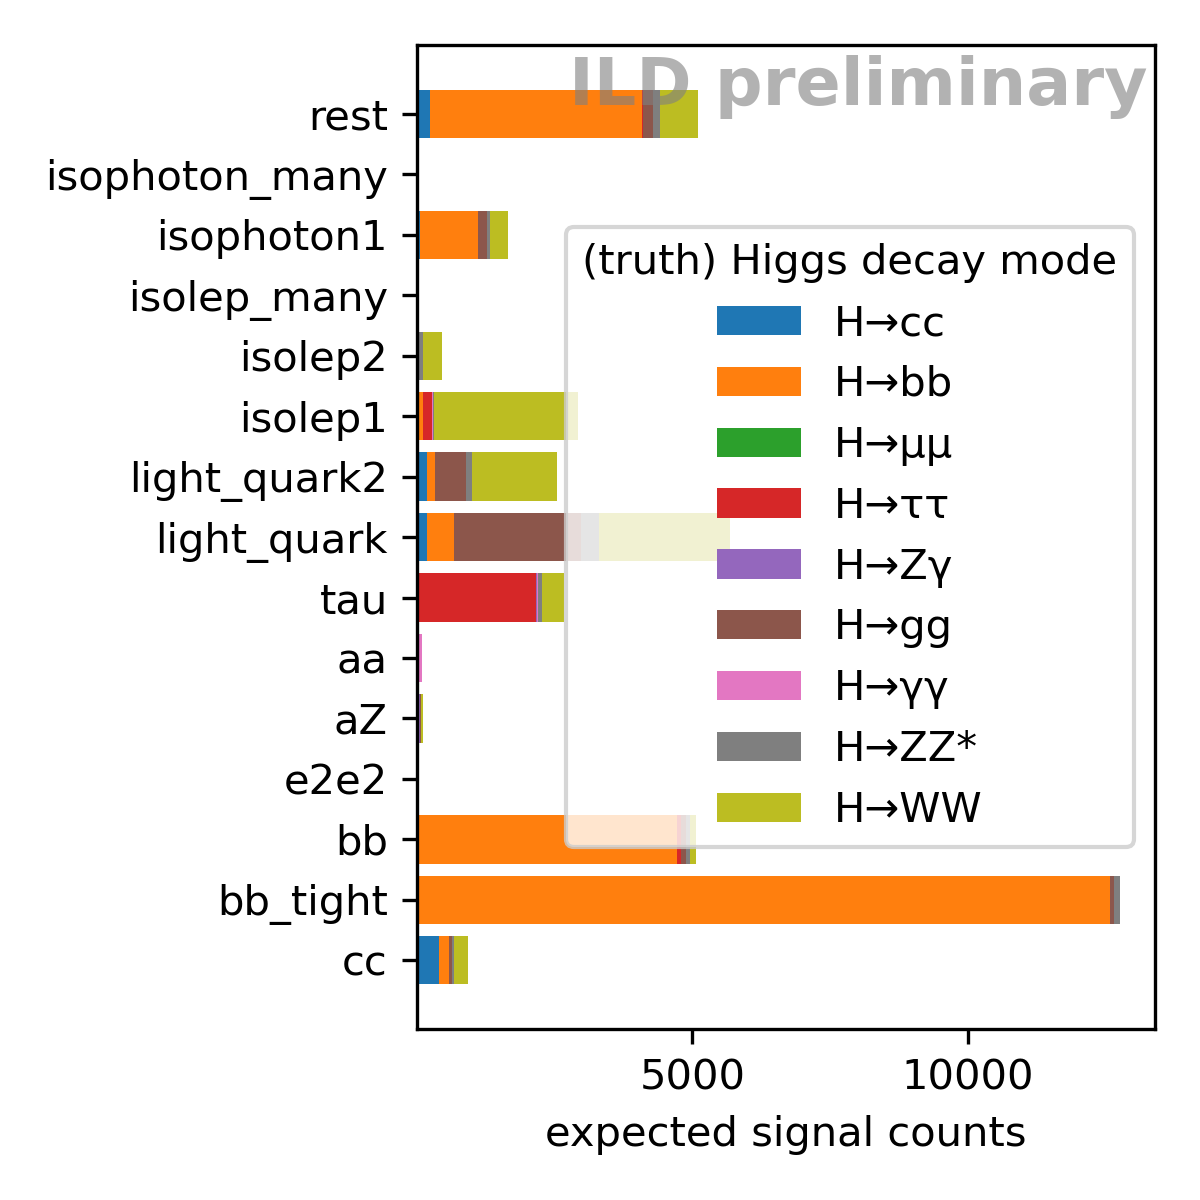
\includegraphics[height=0.85\textheight, width=0.95\textwidth, keepaspectratio]
      {plot_factory/intro_category_counts}}
  \only<4>{\addtocounter{framenumber}{1} 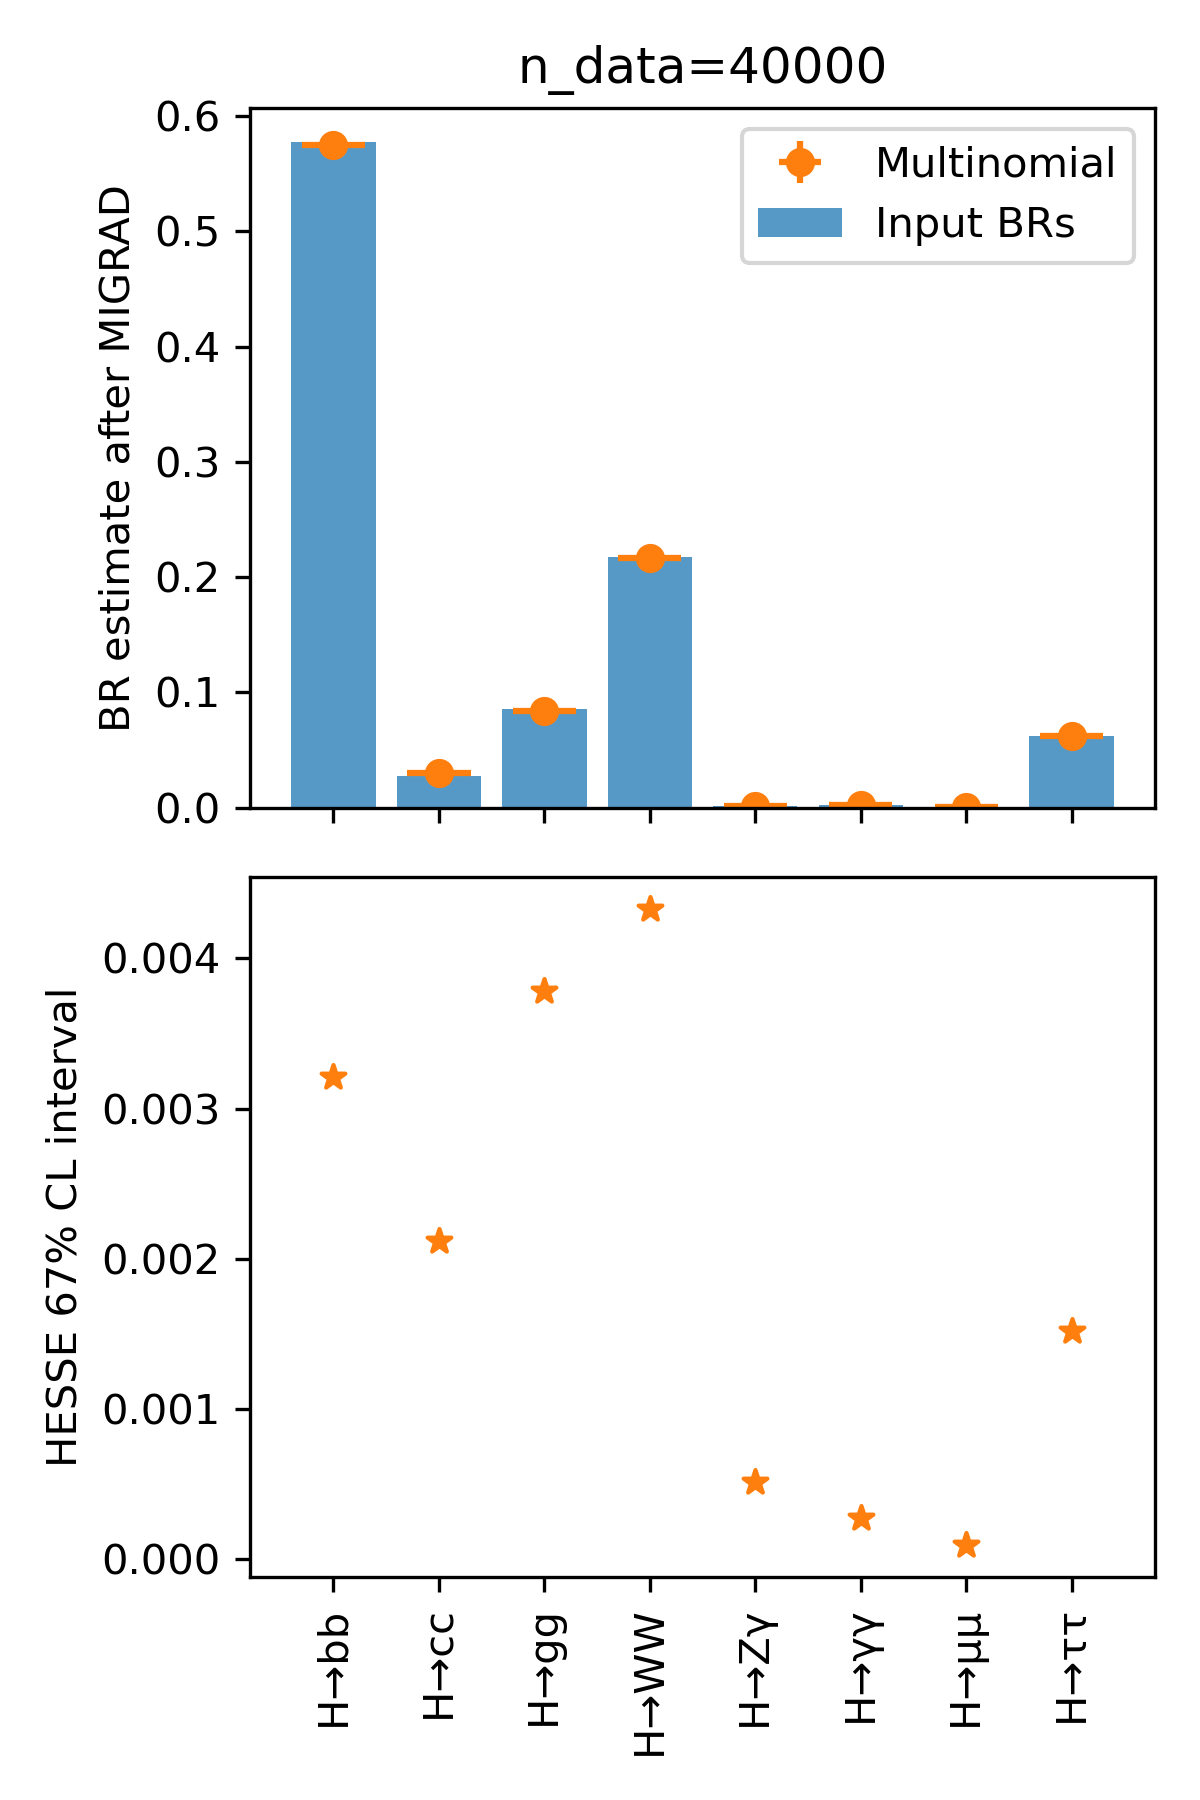
\includegraphics[height=0.85\textheight, keepaspectratio]
      {plot_factory/br_estimates}}
  \only<5>{\addtocounter{framenumber}{1}
    \\
    \textbf{Advantages}
    \begin{itemize}
      \item A model independent extraction of all branching ratios (at once).
      \item Independent of any Higgs production cross section measurement.
      \item Gaussian errors $\rightarrow$ multinomial errors, as everything is in the same sample.
      \begin{itemize}
          \item Promising e.g. for $H \to b\bar{b}$.
                See {\color{llblue}\ref{many_likelihoods_optimizations}} in backup.
      \end{itemize}
    \end{itemize}}
  \end{column}
  \end{columns}
  \end{frame}
